\documentclass{standalone}
\usepackage{tikz}

\usetikzlibrary{calc,math}


\begin{document}

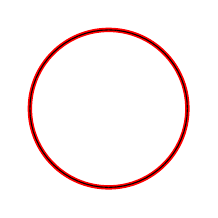
\begin{tikzpicture}
  \tikzmath{
      int \nvertices;
      \nvertices=64;
  }
  \draw[red,ultra thick] (0,0) circle [radius=1];
  \foreach[evaluate={360/\nvertices*\i} as \anglea, evaluate={360/\nvertices*(\i+1)} as \angleb] \i in {1,...,\nvertices} {
    \draw (\anglea:1) -- (\angleb:1);
  }
\end{tikzpicture}

\end{document}